\chapter{Evaluation}
In this chapter, we analyse the performance impact of the IOMMU, directly comparing it to the physical address approach. To compare the both approaches fairly, we dont include allocation and mapping times and perform them upfront. The main focus lies on the IOMMU itself and how it performs with different page sizes. All performance tests use the Container IOMMU API as it currently remains the widely adopted VFIO variant.
Due to the page size limitation of using physical addresses, we cannot compare the IOMMU to physical addresses using \qty{4}{\kibi\byte} pages.

\section{Setup}
We benchmark the performance of the driver on two systems.
Both systems run Ubuntu 23.10 with Linux kernel version 6.5.0-42.
Even though the NVMe Specification supports up to 65536 I/O queues, our SSDs have a maximum of around 64 I/O queues, which seems to be a common amount. We use 1 thread per 1 I/O queue in our multithreaded tests. Turbowrite is a Samsung technology which drastically speeds up write latencies the so called "Turbowrite" buffer with the size of \qty{42}{\giga\byte} of the NVMe, as shown in \cite{vroom}. In order to use the Turbowrite NVMe to its maximum potential, most tests are conducted in said buffer to avoid the NVMe being the bottleneck instead of the IOMMU.
The NVMe SSDs are formatted to 512 Byte blocksize.
Additionally, all standard tests are run with the \texttt{iommu=nomerge} kernel parameter to prevent the IOMMU from merging entries together, which can influence the results.

\begin{table}
    \centering
    \begin{tabular}{lllrll}
        \textbf{CPU}                          & \textbf{Memory}                         & \textbf{NVMe}                         & \textbf{Capacity}                       & \textbf{Count}   \\
        \toprule

        \multirow{2}{*}{Intel Xeon E5-2660v2} & \multirow{2}{*}{\qty{251}{\gibi\byte}}  & \multirow{2}{*}{Samsung Evo 970 Plus} & \multirow{2}{*}{\qty{1}{\tera\byte}}    &
        \multirow{2}{*}{1}                                                                                                                                                                   \\
                                              &                                         &                                       &                                         &                & \\ \hline

        \multirow{2}{*}{AMD EPYC 7713}        & \multirow{2}{*}{\qty{1007}{\gibi\byte}} & \multirow{2}{*}{Samsung PM9A3}        & \multirow{2}{*}{\qty{1.92}{\tera\byte}} &
        \multirow{2}{*}{8}                                                                                                                                                                   \\
                                              &                                         &                                       &                                         &                & \\
        \bottomrule
    \end{tabular}

    \caption{Specifications of systems used in performance testing}
    \label{tab:servers}
\end{table}

\begin{table}
    \centering
    \begin{tabular}{llrrrr}
        \multirow{2}{*}{\textbf{CPU}} & \multirow{2}{*}{\textbf{Clock}} & \multirow{2}{*}{\textbf{Cores}} & \multirow{2}{*}{\textbf{Virtualization}} & \multirow{2}{*}{\textbf{Year}}
        \\
                                      &                                 &                                 &                                          &                                \\
        \toprule

        Intel Xeon E5-2660v2          & \qty{2.2}{\giga\Hz}             & 10                              & VT-d                                     & 2012                           \\
        AMD EPYC 7713                 & \qty{2.0}{\giga\Hz}             & 64                              & AMD-V                                    & 2021                           \\

        \bottomrule
    \end{tabular}

    \caption{CPUs of the systems}
    \label{tab:cpus}
\end{table}

\begin{table}
    \centering
    \begin{tabular}{lrrll}
        \multirow{2}{*}{\textbf{NVMe}} & \textbf{Maximum}     & \textbf{Maximum}    & \multirow{2}{*}{\textbf{Turbowrite}} & \multirow{2}{*}{\textbf{Usage}} \\
                                       & \textbf{Queue Count} & \textbf{Queue Size} &                                      &                                 \\
        \toprule

        Samsung Evo 970 Plus           & 64                   & 16384               & Yes                                  & Consumer                        \\
        Samsung PM9A3                  & 64                   & 16384               & No                                   & Enterprise                      \\

        \bottomrule
    \end{tabular}

    \caption{NVMe(s) of the systems}
    \label{tab:nvmes}
\end{table}

% IOMMU specs, processor, ...

As Linux as well as our IOMMU supports \qty{4}{\kibi\byte}, \qty{2}{\mebi\byte} and \qty{1}{\gibi\byte} page sizes we will test and analyse how it affects the overall performance.

\section{Overall Latency and Throughput}
First, we will compare the VFIO implementation to the MMIO implementation using latency and throughput tests. In these tests, we repeatedly write/read from a \qty{4}{\kibi\byte} buffer in the memory. Each I/O operation uses a \qty{4}{\kibi\byte} unit size.

In these tests, we can see that there is practically a negligable amount of overhead. As this test only uses a one page buffer at maximum, the buffer is constantly stored in the IOTLB.

This test uses one buffer from which the NVMe driver reads/writes to. This buffer and the Queues can fit on the IOTLB. Fetching addresses from the IOTLB is very efficient and thus, no significant performance impact occurs.

\begin{figure}
    \centering
    \subcaptionbox {Random write} {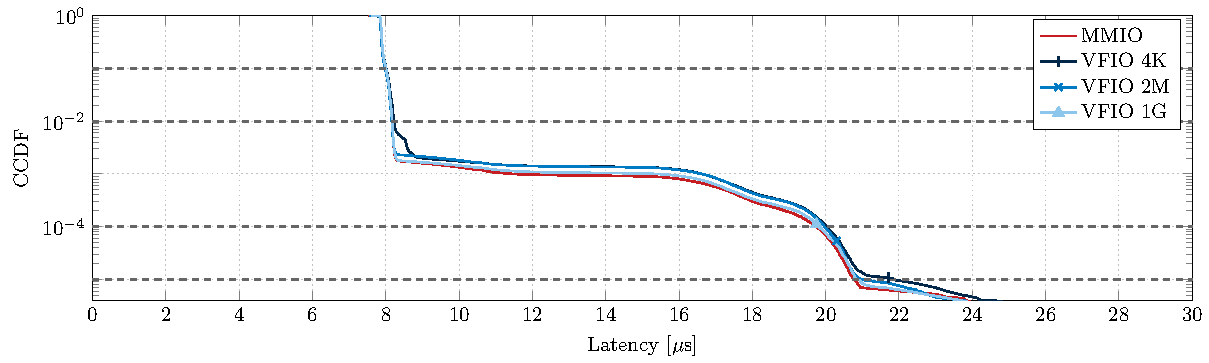
\includegraphics[width=\textwidth]{figures/latency_ccdf_write} \label{fig:ccdf-write}}
    \subcaptionbox {Random read} {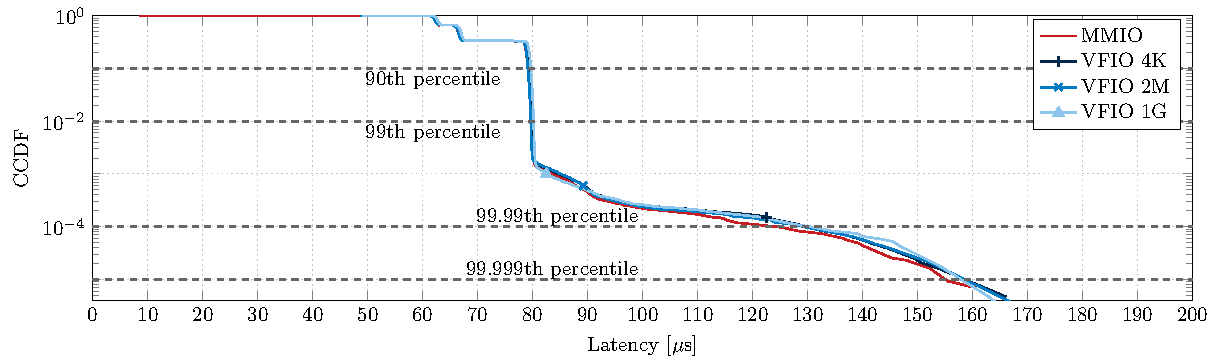
\includegraphics[width=\textwidth]{figures/latency_ccdf_read} \label{fig:ccdf-read}}
    \caption{Tail latencies}
    \label{fig:ccdf}
\end{figure}

\begin{figure}
    \centering
    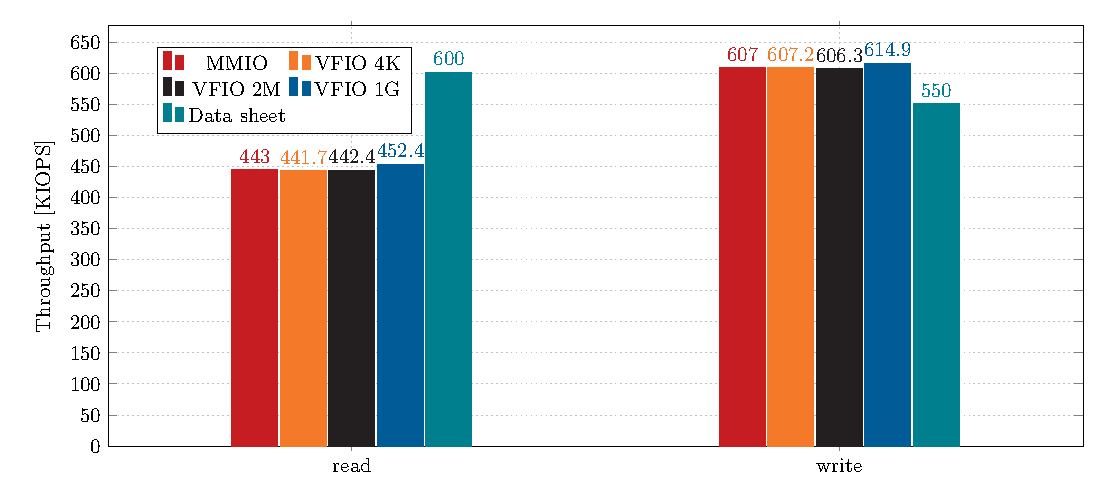
\includegraphics[width=\textwidth]{figures/throughputqd32t1singlepage}
    \caption{Write and Read Operations with queue depth 32 and 4 threads}
    \label{fig:iopsq32t1sp}
\end{figure}

\section{Determining IOTLB size}
As the size of the IOTLB is not stated in hardware and VT-d specifications, we use a latency test to analyse the behaviour of the IOMMU. We can assume that the IOTLB entry count must be a power of two. In order to isolate the effect of the IOMMU we aim to analyse the latencies of the fastest operation the NVMe can perform. The fastest operation is using random writes with the smallest blocksize of \qty{512}{\byte} on an empty NVMe drive. We repeatedly perform this operation on a number of pages that is an increasing power of two. Taking the median and comparing them we can figure out where a latency spike occurs and can then derive the IOTLB size. We configure the queues, buffer and prp-list to each take up one page, resulting in 6 allocated pages before the actual workload. This test is done using without the IOMMU with \qty{2}{\mebi\byte} pages and the IOMMU with \qty{4}{\kibi\byte}, \qty{2}{\mebi\byte} and \qty{1}{\gibi\byte} pages. In order to test \qty{1}{\gibi\byte} pages, we first need to increase the ulimit settings, as memlock limits the amount of locked-in-memory address space.

\paragraph{Results of Intel Xeon}

In the resulting graph \autoref{fig:med-ps} we can observe a performance spike of around 300 nanoseconds for each write between 128 and 256 allocated pages. In the case of \qty{4}{\kibi\byte} pages, this is a memory size of only 512 KiB. Using this information, we can assume that the IOTLB has the same size for each pagesize, as well as it being 128 entries of size.

\begin{figure}
    \centering
    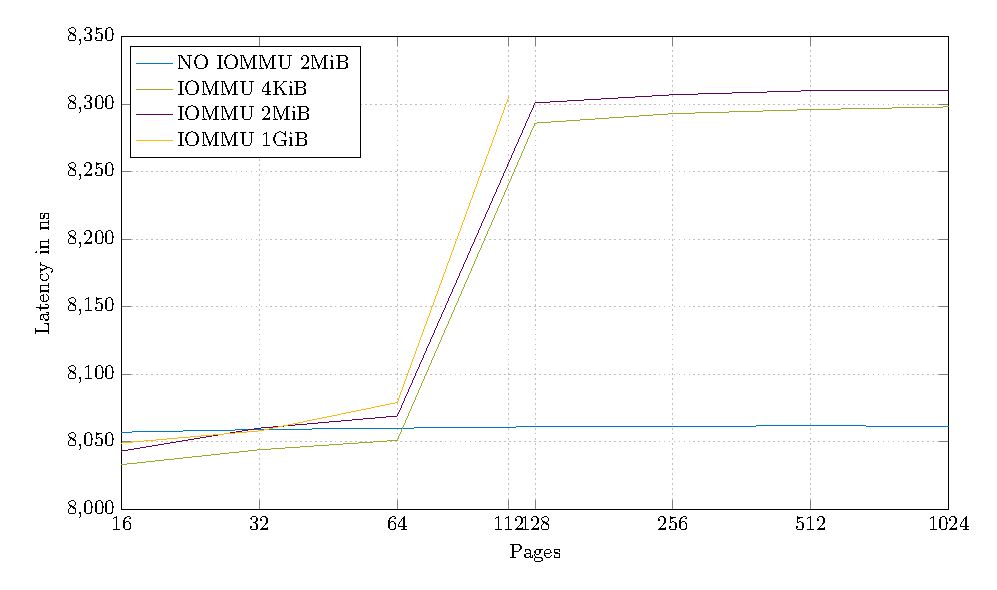
\includegraphics[width=\textwidth]{figures/psmeds}
    \caption{Latencies of random writes on an emptied SSD with increasing host memory pages on the Intel system}
    \label{fig:med-ps}
\end{figure}

\paragraph{Results of AMD Epyc}

On the AMD IOMMU, we can see a performance spike that occurs at 64-128 pages for \qty{2}{\mebi\byte} and \qty{1}{\gibi\byte} page sizes and at 256-512 pages. We can therefore assume that the IOTLB size depends on the pagesize unlike on the Intel CPU. The performance itself only decreases by about \qty{60}{ns}, which is a five fold performance increase of page walks compared to the intel cpu system.

\begin{figure}
    \centering
    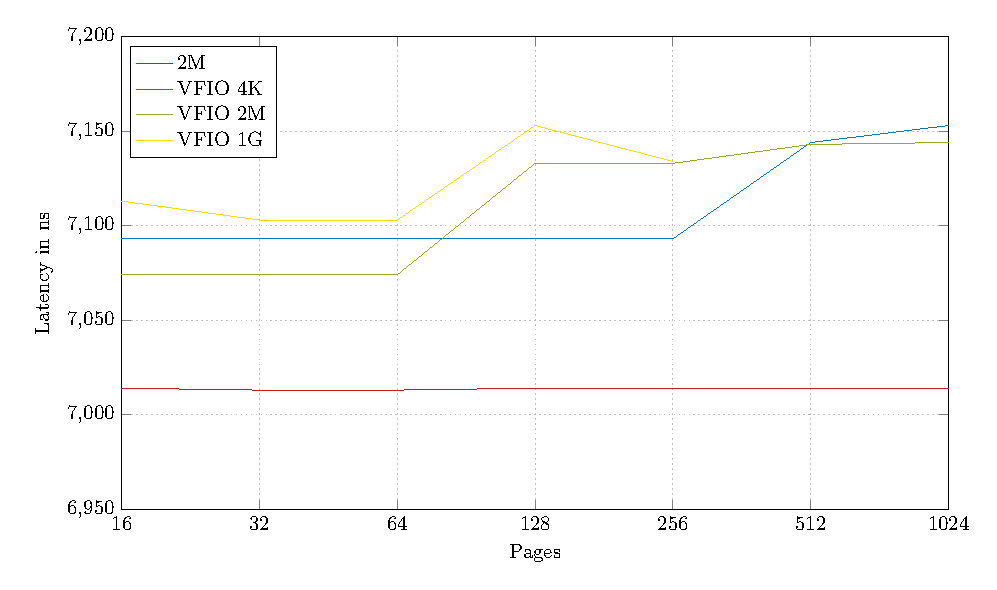
\includegraphics[width=\textwidth]{figures/psmedsepyc}
    \caption{Latencies of random writes on an emptied SSD with increasing host memory pages on the AMD system}
    \label{fig:med-psepyc}
\end{figure}

\section{Multithreaded Random Writes}
When using multithreaded random writes with queue depth 1, in \autoref{fig:qd1tn} we can mostly see the same performance for 1 page, until 32 threads. This is because we allocate a buffer for each thread. For each thread, the submission queue, the completion queue and the buffer take up each one entry of the IOTLB. Therefore, with 32 threads we use 96 pages, exceeding the 64 entries we can store in the IOTLB. Using a \qty{2}{\mebi\byte} buffer, we see around 10\% less performance using \qty{4}{\kibi\byte} pages, as even with one thread, the page count exceeds the possible entries in the IOTLB. The performance of the \qty{2}{\mebi\byte} Vfio implementation stays the same as with 1 \qty{4}{\kibi\byte} buffer, as the \qty{2}{\mebi\byte} buffer fits in one IOTLB entry.

\begin{figure}
    \centering
    \subcaptionbox {1 \qty{4}{\kibi\byte} buffer per thread} {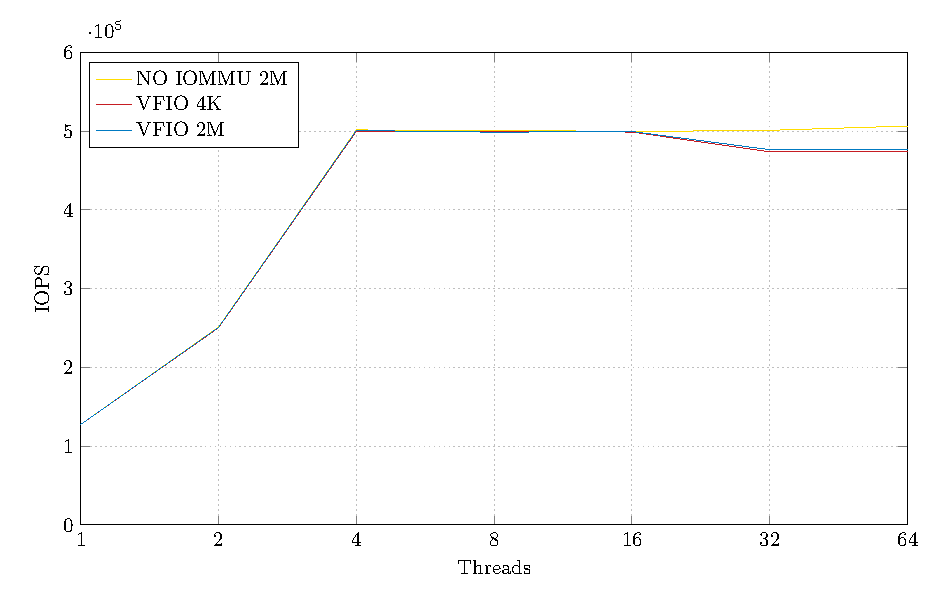
\includegraphics[width=0.75\textwidth]{figures/qd1tn_1page}}
    \subcaptionbox {1 \qty{2}{\mebi\byte} buffer per thread} {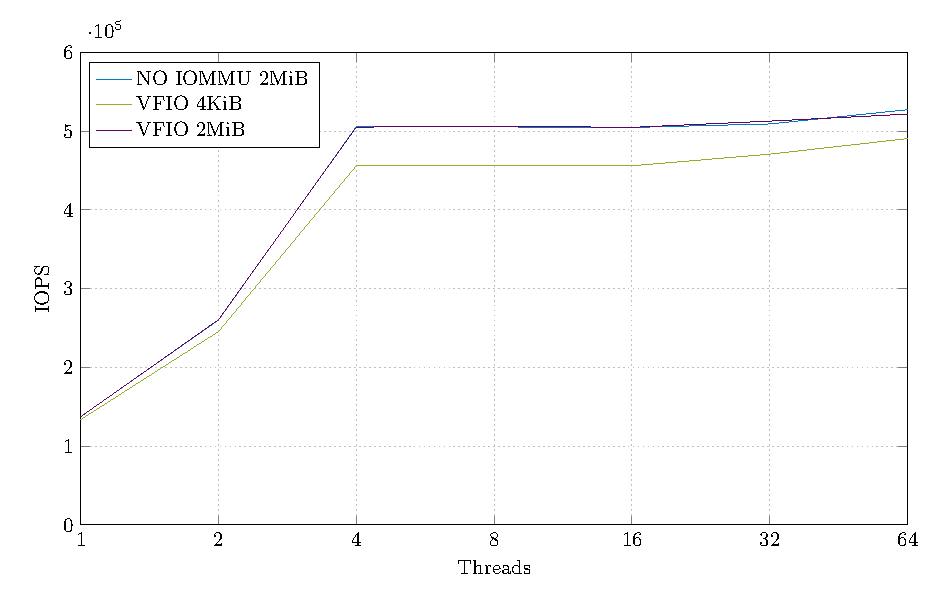
\includegraphics[width=0.75\textwidth]{figures/qd1tn_512page}}
    \caption{QD1 Random Write Throughput with multithreading}
    \label{fig:qd1tn}
\end{figure}

\section{Increasing Queue Depth}
To further test performance we can increase the queue depth. This metric describes how many outstanding commands can be placed on each queue.

\section{Using multiple SSDs}
All tests with multiple SSDs are run on the system with the AMD CPU.

\section{IOMMU modes}
There are a couple of kernel parameters that can be set at boot-time to influence the behaviour of the IOMMU. The availability is influenced by the iommu manufacturer, e.g. theres \texttt{amd\_iommu} and \texttt{intel\_iommu}, as well as the CPU architecture. Many of these manufacturer dependent options are either very specific, or shared behaviour is ported to the general iommu parameter, e.g. \texttt{amd\_iommu=fullflush} and \texttt{intel\_iommu=strict}. We will be mainly looking at the general options \texttt{iommu}.

\paragraph{Strict}
To enable strict IOMMU mode, \texttt{iommu.strict=1} has to be set. Using strict mode, unmapping operation cause a complete IOTLB invalidation. Using relaxed mode, unmapping operations can be deferred and batched. This increases performance as an invalidation completely clears the IOTLB buffer, but reduces device isolation.

\paragraph{Passthrough}
Passthrough mode can be enabled using \texttt{iommu.passthrough=1}. Using passthrough DMA operations bypass the translation of the IOMMU, and instead directly access physical memory.